\chapter{Event Selection}\label{chapt:event_sel}
 
This work is aiming to reconstruct the $t\bar{t}$ pair in the dilepton decay channel, or
$t\bar{t} \to W^{+}b\,W^{-}\bar{b} \to \bar{l}\nu b\,l\bar{\nu}\bar{b}$, thus 
looking for events in the detector with two leptons of different sign and two jets. The 
neutrino can't be measured directly, their presence is reflected by a non-zero transverse
missing energy $E_{T}^{miss}$. The low branching ratio of the dileptonic decay channel
($BR \simeq 4.8\%$) is compensated by an excellent lepton identification and reconstruction, 
which reduces the fraction of background events to large extent.

The reconstructed objects in each event (which corresponds to one bunch crossing) have to fulfill certain 
criteria to be accepted for this analysis. These criteria are chosen taking to account the physical 
result this analysis is aiming for and the technical features of the CMS detector parts.

The imperfect correspondence of the simulation model to the real data has to be additionally 
corrected. The differences in efficiencies of certain procedures in data and simulation 
are corrected by applying \textit{Scale Factors}, $SF = \frac{\epsilon_{data}}{\epsilon_{MC}}$, 
on the MC distributions. Here $\epsilon_{data}$ is the efficiency determined in the experimental 
data and $\epsilon_{MC}$ is the efficiency from simulation. 

This chapter gives an overview of the $t\bar{t}$ event selection. The 
procedures are based on the CMS Top-Quark-Physics-Analysis group recommendations \cite{TopPAGreco}.
The full chain of event selection is described. 
Resulting event yields are represented in control distributions, showing the data, simulated signal and backgrounds.

\section{Background Sources}\label{sec:bg_intro}

Not all of the events which have two identified leptons and two jets in the final state are signal events
originating from the $t\bar{t}$ system decay in dileptonic channel. Events may arise from different processes, 
called \textit{background} for the specific measurement. In this analysis the background rates are estimated 
from the simulation. The following background processes are relevant for this analysis:

\begin{itemize}
 \item $t\bar{t}\rightarrow$other. This background source includes the other $t\bar{t}$ decay modes (see sec. \ref{ssec:tdecay}).
 This background source is dominated by the semileptonic channel as it contains a lepton in the final state;
 \item single top production, which was simulated using \Powheg + \PYTHIA. A top is produced in association with a $W$ boson, which can be 
 mistreated as a $W$ boson from the top decay;
 \item Drell-Yan processes, $Z/\gamma^{*} \rightarrow \tau\tau$ and $Z/\gamma^{*} \rightarrow ee/\mu\mu$, which ware generated utilizing \PYTHIA. 
 Since they also has a dileptonic final state signature, they can be misidentified as $t\bar{t}$ signal. However, only same flavour leptons 
 are produced in Drell-Yan processes. Therefore, the fraction of these
 background events in the $e\mu$ final state is small;
 \item $WW$, $WZ$, $ZZ$ diboson production, simulated using \PYTHIA. These events can also have a dileptonic final state and may be 
 picked as a $t\bar{t}$ candidate;
 \item associated $t\bar{t}\;+\; W/Z/\gamma$ production, simulated with \MG + \PYTHIA. For this process one expects only one ore none 
 hard leptons in the final state. However, the production rates are high and occasionally one or two leptons, which originate from hadron
 decays or from hadrons misidentified as leptons, can be picked up;
 \item associated $W\;+\;jets$ production, generated using \MG + \PYTHIA. The reason why this process can be misidentified as a $t\bar{t}$
 production is similar to the previous case;
 \item QCD multijet processes, generated with \PYTHIA.
\end{itemize}

The simulated background samples were normalized to the data integrated luminosity of 19.7 fb$^{-1}$ and
scaled to the total cross sections predicted by higher order calculations\cite{TWikiXSec}.

Whereas all the other background yields are only simulated, the estimated total rate of the background caused by Drell-Yan production is 
partially data driven \cite{Chatrchyan:2011nb}. The normalization factor for the simulated Drell-Yan events is determined 
from the comparison of the reconstructed and the simulated $Z$-peak in the clean decays $Z \rightarrow ee/\mu\mu$. 

The selection, which will be introduced in this section, is aiming to distinguish the $t\bar{t}$ events
from the background processes exploiting physical features of each process.

\section{Good Runs}

For the work presented in this thesis the following CMS data samples were used:

\begin{center}\label{tab:samples}
  \begin{tabular}{| c c c |}
    \hline
    \textbf{Samples} & \textbf{Events} & \textbf{Run Range} \\ \hline
    /MuEG/Run2012A-22Jan2013-v1/AOD & 2.5M & 190456 - 193621 \\ 
    /MuEG/Run2012B-22Jan2013-v1/AOD & 15M & 193834 - 196531 \\
    /MuEG/Run2012C-22Jan2013-v1/AOD & 21M & 198022 - 203742 \\
    /MuEG/Run2012D-22Jan2013-v1/AOD & 22M & 203777 -  208686 \\
    \hline
  \end{tabular}
\end{center}

Only the good runs from the LHC certified good run list\cite{JSON} are selected for the analysis out of these data sets.

\section{$t\bar{t}$ Event Selection and Correction}\label{sec:sel}

The analysis follows closely a previous measurement selection strategy described in \cite{Asin2014Auth}. Various selection criteria and related scale factors are presented in this section.

The results of the selection are presented in the control distributions. These plots show the comparison between the yields in the experimental data and the simulated MC samples.
% The various background sources are also presented separately in the distributions. 
% The simulated yields are additionally scaled to the data luminosity of 19.7\;fb$^{-1}$.
All the plots include the statistical uncertainties only.

All the selection requirements are summarized as follows:

\begin{itemize}
 \item [--] \textbf{Trigger selection}: The events have to be accepted by the HLT (see section \ref{sec:trig}) dilepton triggers, which require the presence of two leptons, electron and muon, with
 minimum transverse momentum of 17 GeV and 8 GeV, respectively.
 
 As the triggers may perform with different efficiencies for the data and for MC, the scale factor corrections were applied. As all the data taken in the detector is being selected by 
 at least one trigger, there is no ``reference'' data before the trigger selection. That is why the efficiency of the particular trigger can be determined only with respect to another
 spectator trigger. A spectator should be as independent from the tested trigger as possible. The efficiencies for the trigger scale factors in this work were 
 determined using the $E_{T}^{miss}$-based trigger as a spectator \cite{Asin2014Auth}. The scale factors connected to the trigger selection were applied on the MC 
 double differentially in bins of the two leptons pseudorapidities. 
 %%%% 
 \item [--] \textbf{Beam scrapping}: Accept only events with maximum 10 reconstructed tracks, or more than 10 in case at least quarter of them has high quality of reconstruction.
 %%%%
 \item [--] \textbf{Calorimeter noise removal}: Event with anomalous calorimeter noise are removed.
 %%%%
 \item [--] \textbf{Vertex requirement}: Events with at least one "good" primary vertex are selected.
 This means that the number of associated tracks should be larger then 4 and a vertex should be positioned centrally in the detector
 \footnote{Only the events with a vertex position $|z| < \textrm{24 cm}$ and $|\rho| = |\sqrt{x^{2} + y^{2}}| < \textrm{2 cm}$ are accepted. All the coordinates
 are given with respect to the CMS coordinate system (see sec.\ref{sec:CMS})}. Only the ``hardest vertex'' 
 (with the highest sum of the $p_{T}^{2}$ of the assigned tracks) is taken for the analysis. 
 \\
 The distribution of the number of secondary vertices differs in the data and in the MC. The weight correction depending on the event vertex multiplicity is applied
 event-by-event on the MC to make it match the data distribution.
 The Fig. \ref{fig:PUweight} shows how the agreement
 between the experimental and simulated data improves after this reweighting is implemented.
 
 \begin{figure}[h]
 \centering
 \begin{subfigure}
   \centering
   \includegraphics[width=0.49\textwidth]{/home/dolinska/Dropbox/desy_plots/Thesis/Jenya/04_event_selection/PileUPw/Nominal/emu/vertMulti_noPU.pdf}
 \end{subfigure}
 \begin{subfigure}
   \centering
   \includegraphics[width=0.49\textwidth]{/home/dolinska/Dropbox/desy_plots/Thesis/Jenya/04_event_selection/PileUPw/Nominal/emu/vertMulti_PU.pdf}
 \end{subfigure}
 \caption{The vertex multiplicity control distribution before (left) and after (right) the vertex correction reweighing after the full event selection.
 Black dots represent the experimental data and the colored histograms are the MC simulation divided into signal and backgrounds contributions.
 The bottom plots represent the ratio between experimental and simulated data rates.}
 \label{fig:PUweight}
 \end{figure}
 
 %%%%%
 \item [--] \textbf{Lepton isolation}: All the leptons in the event have to be isolated with $I_{rel}\leq 0.15$ in a cone of $\Delta R = \sqrt{\Delta\eta^{2} + \Delta\phi^{2}} = 0.3$ 
 around the lepton track, where $I_{rel}$ is the relative isolation defined as:
  \begin{equation}\label{eq:Iso}
   I_{rel} = \frac{\sum E_{Tracker} + \sum E_{ECAL} + \sum E_{HCAL}}{p_{T}(l)}
  \end{equation}
 
 As it is shown in the Fig. \ref{fig:PFIso}, the lepton isolation requirement cuts mainly on the QCD background.

 \begin{figure}[h]
 \centering
 \begin{subfigure}
   \centering
   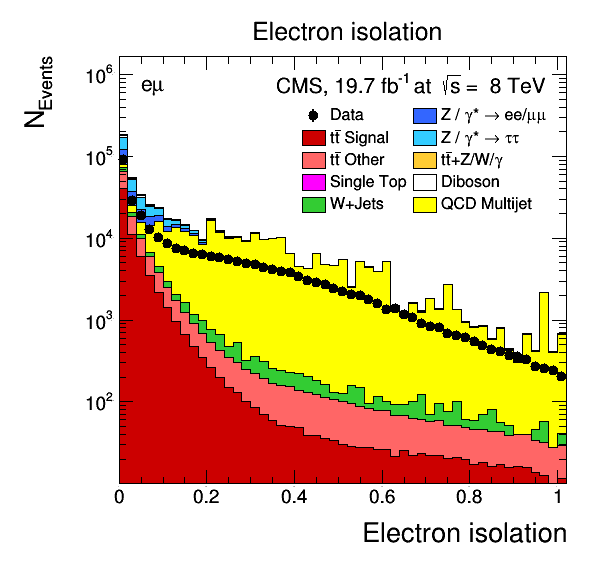
\includegraphics[width=0.49\textwidth]{/home/dolinska/Dropbox/desy_plots/Thesis/Jenya/04_event_selection/PFiso/Plots/Nominal/emu/PF_e_Iso.pdf}
 \end{subfigure}
 \begin{subfigure}
   \centering
   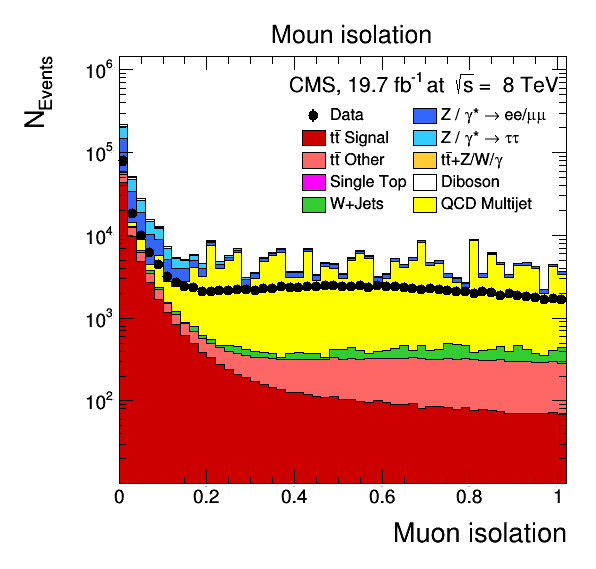
\includegraphics[width=0.49\textwidth]{/home/dolinska/Dropbox/desy_plots/Thesis/Jenya/04_event_selection/PFiso/Plots/Nominal/emu/PF_mu_Iso.pdf}
 \end{subfigure}
 \caption{Control distribution electron (left) and muon (right) relative isolation ($I_{rel}$) (\ref{eq:Iso}) after the trigger selection. The experimental data points (black dots)
  and simulated distributions (colored histograms) of signal and different backgrounds are shown. The error bars of the data points
  correspond to the statistical uncertainties. The bottom plot represent the data-to-MC yield ratio distributions. The vertical dashed lines show the isolation cut value.}
 \label{fig:PFIso}
 \end{figure}
 
 The efficiencies of the lepton isolation were determined using a \textbf{tag and probe} method \cite{TWikiTP}. The corresponding scale factors are applied on the
 simulation level in bins of $p_{T}$ and $\eta$ of lepton separately for electrons and for muons.
 %%%%%
 \item [--] \textbf{Lepton pair selection}: An event has to contain at least two opposite signed leptons (electron-muon pair) with $p_{T} > 20 \; \textrm{GeV}$ and $|\eta| < 2.4$.
 The invariant mass of the system of the leading $p_{T}$ electron and muon has to be more than 20 GeV, otherwise the event is rejected. In the following analysis steps
 only the leading $p_{T}$ leptons are considered.
 %%%%%
 \item [--] \textbf{Jets selection}: Events which contain at least two jets with $p_{T} > 30$ GeV and $|\eta| \leq 2.4$ are accepted. It is natural to expect
 that events with less than two jets will be dominated by Drell-Yan background as the leading order Drell-Yan process does not contain jets in the final state. This is also 
 reflected by the jet multiplicity distribution (Fig. \ref{fig:jetMultiSel}). 
 
 \begin{figure}[h]
  \centering
  \includegraphics[width=0.49\textwidth]{/home/dolinska/Dropbox/desy_plots/Thesis/Jenya/04_event_selection/diLep_mass_jet_mult_bjet_mult/Nominal/emu/basic_jet_multiplicity_step4.pdf}
  \caption{Control distribution of the jet multiplicity in events after the trigger and lepton selection. The experimental data points (black dots)
  and simulated distributions (colored histograms) of signal and different backgrounds are shown. The error bars of the data points
 correspond to the statistical uncertainties. The bottom plot represent the data-to-MC yield ratio distributions. The vertical dashed line shows cut value on the jet multiplicity.}
  \label{fig:jetMultiSel}
 \end{figure}
 
%  In the figure \ref{fig:mllJetSel} the dilepton mass before and after jet selection is shown, demonstrating a sizable background (especially Drell-Yan) fraction suppression power
%  of the cuts implemented in this selection step.
%  
%  \begin{figure}[h]
%  \centering
%  \begin{subfigure}
%    \centering
%    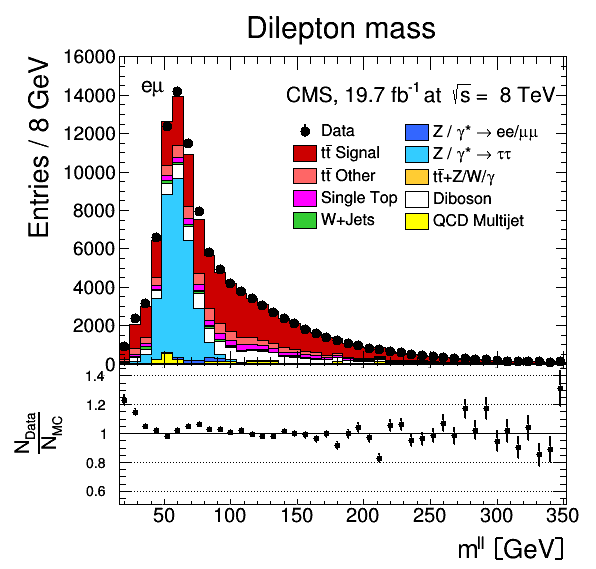
\includegraphics[width=0.49\textwidth]{04_event_reconstruction/plots/mll_step4.png}
%  \end{subfigure}
%  \begin{subfigure}
%    \centering
%    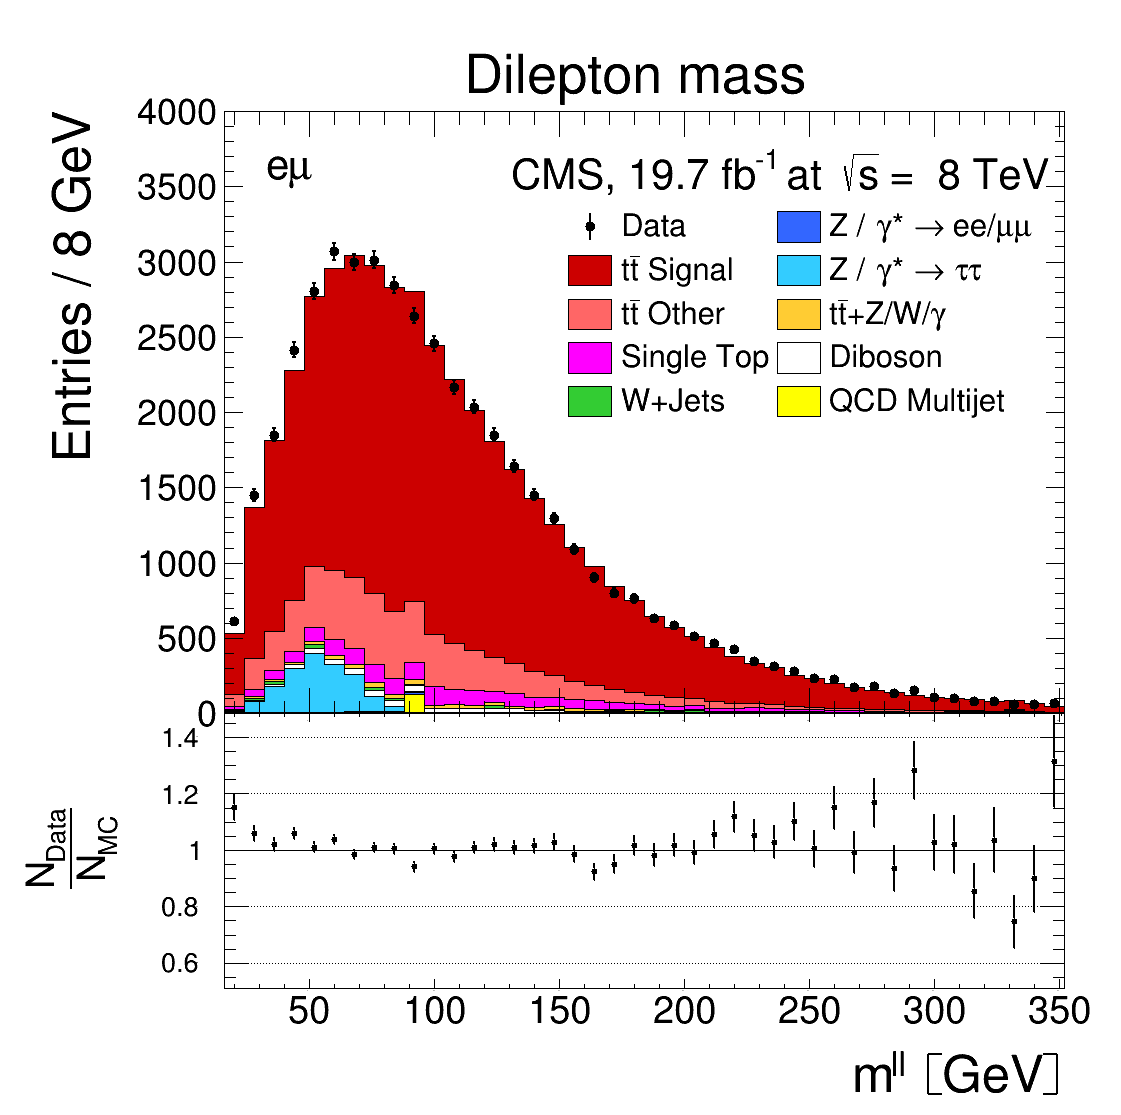
\includegraphics[width=0.49\textwidth]{04_event_reconstruction/plots/mll_step5.png}
%  \end{subfigure}
%  \caption{Control distribution of the dilepton mass in the events after the trigger and lepton selection (left) and after trigger, lepton and jet selection (right). 
%  The experimental data points and simulated distributions of signal and different background are plotted.}
%  \label{fig:mllJetSel}
%  \end{figure}
 %
 \item [--] \textbf{$b$-jets selection}: An event has to contain at least one jet, tagged as originating from a $b$-quark with $b$-tagging probability according to the CSVL cut criterion (sec. \ref{ssec:bTag}). 
 The multiplicity of the $b$-tagged jets is presented in Fig. \ref{fig:bjetMultiSel} which shows that cutting the events with no $b$-tagged jets should remove a sizable background fraction. 
 Indeed, Fig. \ref{fig:mllbJetSel} presenting the dilepton mass before and after the $b$-jets selection shows this background reduction.
 
 \begin{figure}[h]
  \centering
  \includegraphics[width=0.49\textwidth]{/home/dolinska/Dropbox/desy_plots/Thesis/Jenya/04_event_selection/diLep_mass_jet_mult_bjet_mult/Nominal/emu/basic_bjet_multiplicity_step5.pdf}
  \caption{Control distribution of the $b$-jet multiplicity in events after the trigger and lepton selection. The experimental data points (black dots)
  and simulated distributions (colored histograms) of signal and different backgrounds are shown. The error bars of the data points
 correspond to the statistical uncertainties. The bottom plot represent the data-to-MC yield ratio distributions. The vertical dashed line shows the cut value on the $b$-jet multiplicity.}
  \label{fig:bjetMultiSel}
  \end{figure}
  
 \begin{figure}[h]
 \centering
 \begin{subfigure}
   \centering
   \includegraphics[width=0.49\textwidth]{/home/dolinska/Dropbox/desy_plots/Thesis/Jenya/04_event_selection/diLep_mass_jet_mult_bjet_mult/Nominal/emu/basic_dilepton_mass_step6.pdf}
 \end{subfigure}
 \begin{subfigure}
   \centering
   \includegraphics[width=0.49\textwidth]{/home/dolinska/Dropbox/desy_plots/Thesis/Jenya/04_event_selection/diLep_mass_jet_mult_bjet_mult/Nominal/emu/basic_dilepton_mass_step7.pdf}
 \end{subfigure}
 \caption{Control distribution of the dilepton mass in events after the trigger, lepton and jet selection (left) and after applying in addition the $b$-jet selection (right). 
 The experimental data points (black dots) and simulated distributions (colored histograms) of signal and different backgrounds are shown. The error bars of the data points
 correspond to the statistical uncertainties. The bottom plot represent the data-to-MC yield ratio distributions.}
 \label{fig:mllbJetSel}
 \end{figure}
 
 The scale factors corresponding to the $b$-tagging procedure are measured by the BTV group \cite{CMS-PAS-BTV-13-001} for $b$, $c$ and light jets. These scale factors were applied on the MC 
 improving much the agreement between data and simulation. This effect can be seen in the 
 Fig. \ref{fig:bTagDiscr}, which presents the CSV discriminator distribution before and after the $b$-tagging SF reweighing. The data-to-MC ratio plots are getting closer to one with
 applying the SFs.
 
 \begin{figure}[h]
 \centering
 \begin{subfigure}
   \centering
   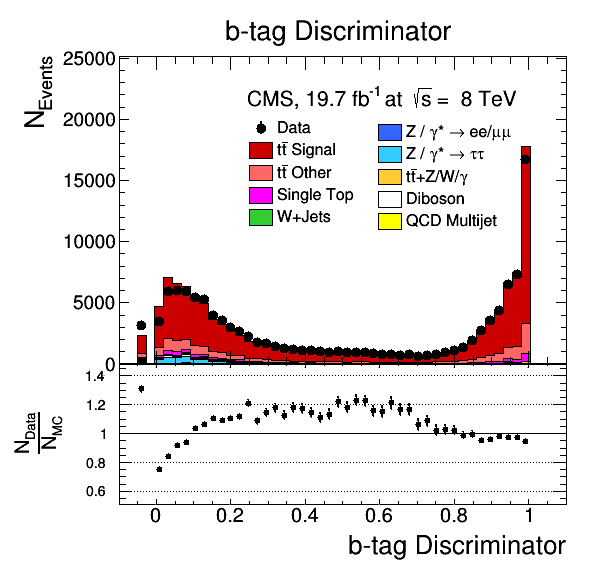
\includegraphics[width=0.49\textwidth]{04_event_reconstruction/plots/bTagDiscr_step6.png}
 \end{subfigure}
 \begin{subfigure}
   \centering
   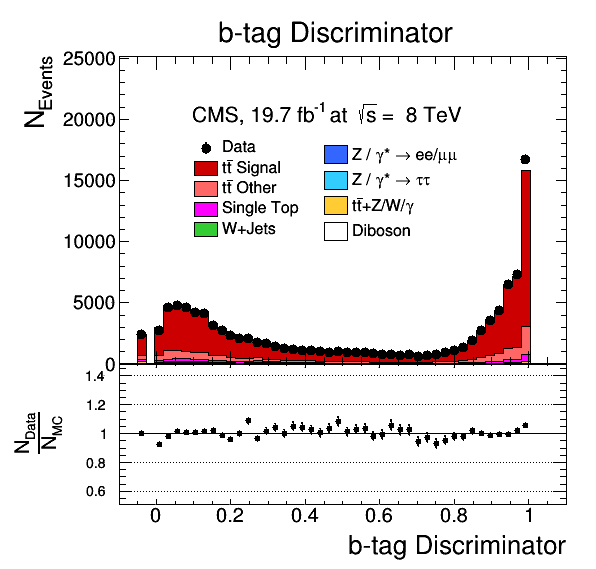
\includegraphics[width=0.49\textwidth]{04_event_reconstruction/plots/bTagDiscr_step7.png}
 \end{subfigure}
 \caption{Control distribution of the $b$-tag discriminator in events after the full even selection (\ref{sec:sel}) not applying the $b$-tag scale factors (left)
 and after applying the $b$-tag scale factors (right). The experimental data points (black dots)
 and simulated distributions (colored histograms) of signal and different backgrounds are shown. The error bars of the data points
 correspond to the statistical uncertainties. The bottom plot represent the data-to-MC yield ratio distributions.}
 \label{fig:bTagDiscr}
 \end{figure}
 %
 \end{itemize}

The applied selection criteria dramatically reduce the fraction of background events, while retaining a large fraction of the signal.

\section{Control Distributions}

The results of the selection described above can be illustrated by control distributions of the objects which are reconstructed for the $t\bar{t}$
final state definition.

The Fig. \ref{fig:CPetaptLep} shows the lepton $\eta$ and $p_{T}$. An overall reasonable agreement between the data and simulation shapes is observed in all $\eta$ regions
and $p_{T}$'s. The control distribution of the mass of the leading dilepton (electron-muon) system is shown in Fig. \ref{fig:CPmll}. The simulation and experimental data
agree well within the statistical uncertainties except for the first bin where data are higher than simulation.

 \begin{figure}[h]
 \centering
 \begin{subfigure}
   \centering
   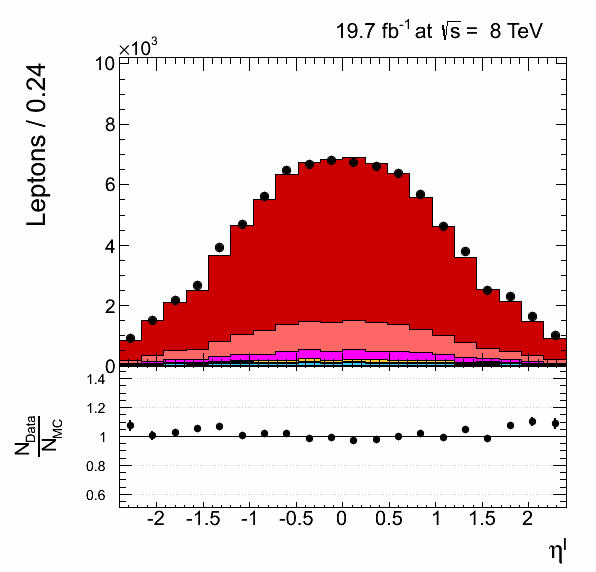
\includegraphics[width=0.49\textwidth]{/home/dolinska/Dropbox/desy_plots/Thesis/Jenya/04_event_selection/Plots-CPs-step7/Nominal/emu/basic_lepton_eta_step7.pdf}
 \end{subfigure}
 \begin{subfigure}
   \centering
   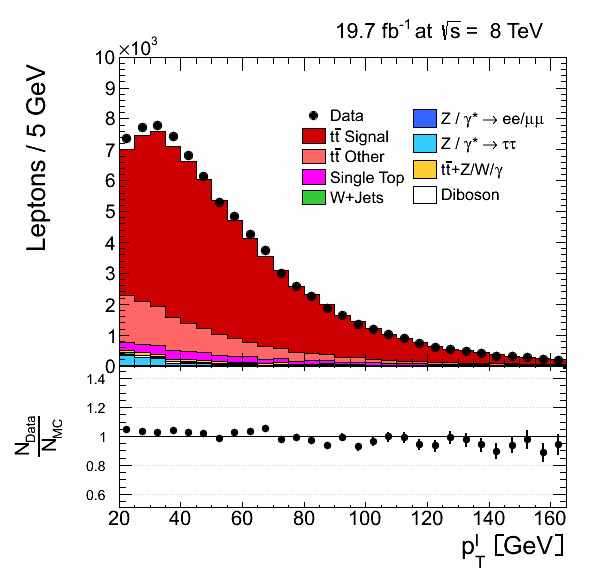
\includegraphics[width=0.49\textwidth]{/home/dolinska/Dropbox/desy_plots/Thesis/Jenya/04_event_selection/Plots-CPs-step7/Nominal/emu/basic_lepton_pt_step7.pdf}
 \end{subfigure}
 \caption{Control distribution of lepton $\eta$ (left) and lepton $p_{T}$ (right) in events after the whole event selection described in sec. \ref{sec:sel}. 
 The experimental data points (black dots)
 and simulated distributions (colored histograms) of signal and different backgrounds are shown. The error bars of the data points
 correspond to the statistical uncertainties. The bottom plot represent the data-to-MC yield ratio distributions.
 Each distribution has two entries per event - one for the electron and one for the muon.}
 \label{fig:CPetaptLep}
 \end{figure}
%  
%  \begin{figure}[h]
%   \centering
%   \includegraphics[width=0.6\textwidth]{04_event_reconstruction/plots/basic_dilepton_mass_step7.png}
%   \caption{Control distribution of the mass of the electron-muon system in events after the whole event selection described in sec. \ref{sec:sel}. 
%   The experimental data points and simulated distributions of signal and different background are plotted. The jets $p_{T}$ and multiplicity 
%   distributions are presented in the logarithmic scale. The error bars of the data points
%   correspond to the statistical uncertainties of the measurement. The bottom plots represent the data-to-MC yield ratio distributions.}
%   \label{fig:CPmll}
%  \end{figure}
 
The kinematics of the reconstructed and selected jets is presented in the Fig. \ref{fig:CPjetskin} which shows the control distributions for the
jets $\eta$, $p_{T}$ and the jet multiplicity in the events. The simulation describes better the central rapidity ranges. For the jet multiplicities
smaller than 5 a good agreement between experimental data and MC is observed.
 
 \begin{figure}[h]
  \centering
  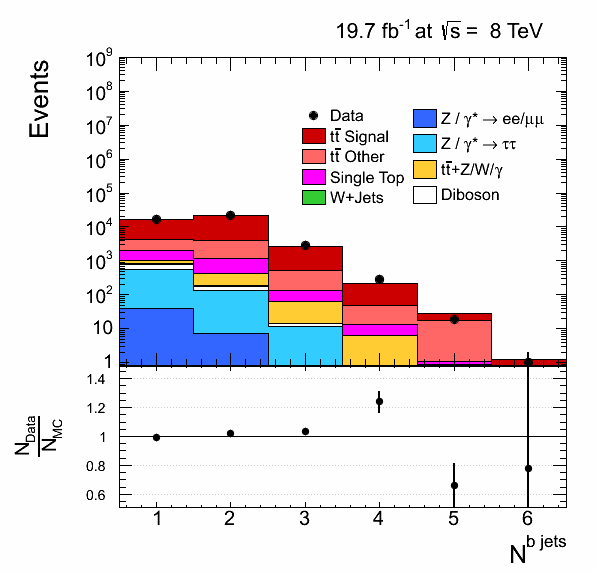
\includegraphics[width=0.49\textwidth]{/home/dolinska/Dropbox/desy_plots/Thesis/Jenya/04_event_selection/Plots-CPs-step7/Nominal/emu/basic_bjet_multiplicity_step7.pdf}
  \caption{Control distribution the $b$-tagged jets multiplicities in events after the whole event selection described in sec. \ref{sec:sel}. 
  The experimental data points (black dots)
  and simulated distributions (colored histograms) of signal and different backgrounds are shown. The error bars of the data points
  correspond to the statistical uncertainties. The bottom plot represent the data-to-MC yield ratio distributions.}
  \label{fig:CPbJetMult}
 \end{figure}
 
 \begin{figure}[h]
 \centering
 \begin{subfigure}
   \centering
   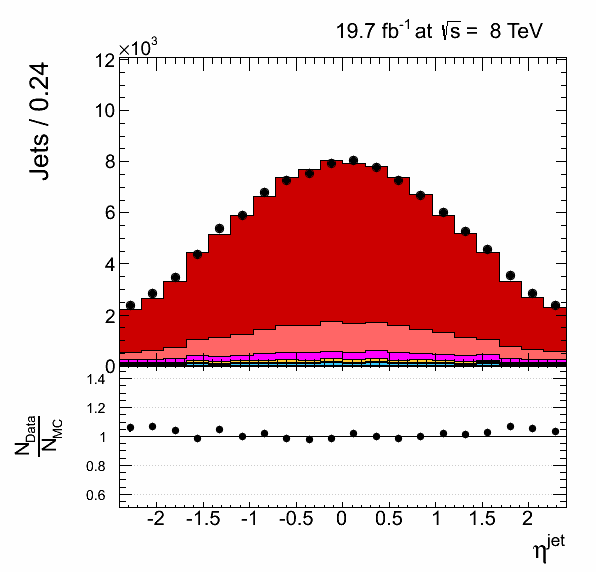
\includegraphics[width=0.49\textwidth]{/home/dolinska/Dropbox/desy_plots/Thesis/Jenya/04_event_selection/Plots-CPs-step7/Nominal/emu/basic_jet_eta_step7.pdf}
 \end{subfigure}
 \begin{subfigure}
   \centering
   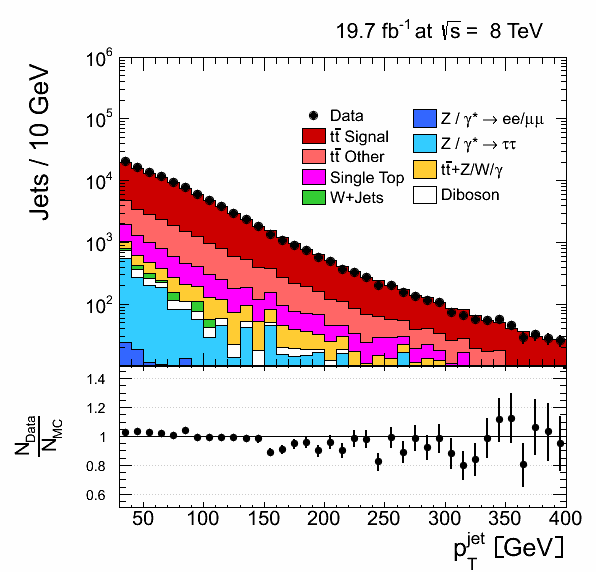
\includegraphics[width=0.49\textwidth]{/home/dolinska/Dropbox/desy_plots/Thesis/Jenya/04_event_selection/Plots-CPs-step7/Nominal/emu/basic_jet_pt_step7.pdf}
 \end{subfigure}
  \begin{subfigure}
   \centering
   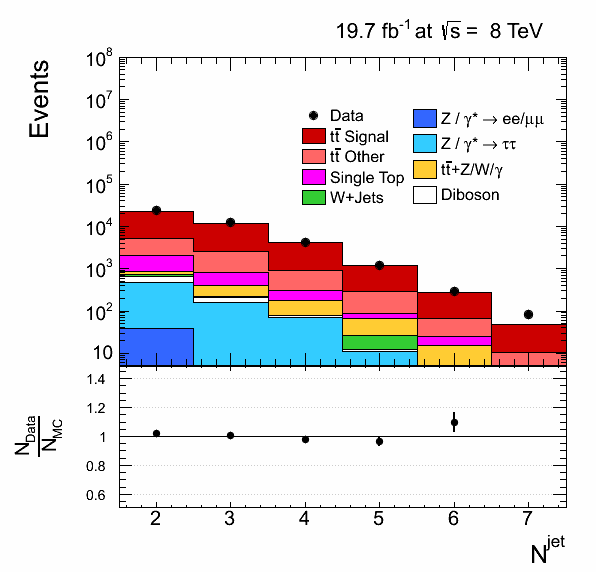
\includegraphics[width=0.49\textwidth]{/home/dolinska/Dropbox/desy_plots/Thesis/Jenya/04_event_selection/Plots-CPs-step7/Nominal/emu/basic_jet_multiplicity_step7.pdf}
 \end{subfigure}
 \caption{Control distribution the jet $\eta$ (top left) and jet $p_{T}$ (top right) for all selected jets and the jet multiplicity in events 
  after the whole event selection described in sec. \ref{sec:sel}. 
  The experimental data points (black dots)
  and simulated distributions (colored histograms) of signal and different backgrounds are shown. The error bars of the data points
  correspond to the statistical uncertainties. The bottom plot represent the data-to-MC yield ratio distributions.
  The top distributions have multiple entries per event, corresponding to all reconstructed jets.}
 \label{fig:CPjetskin}
 \end{figure}
 
The multiplicity for the $b$-tagged jets is presented in Fig. \ref{fig:CPbJetMult} which shows a good agreement for the multiplicities smaller than 4.
 
The control distributions are signal dominated which shows a good performance of the criteria for the $t\bar{t}$ final state selection.



